\documentclass{beamer}

\beamertemplatenavigationsymbolsempty

\mode<presentation>
{
  \usetheme{default}
}

\usepackage[english]{babel}
\usepackage[latin1]{inputenc}
\usepackage{bussproofs}

% needs debian package texlive-math-extra
\usepackage{stmaryrd} % for \llbracket, \rrbracket

\usepackage{times}
\usepackage[T1]{fontenc}
% Or whatever. Note that the encoding and the font should match. If T1
% does not look nice, try deleting the line with the fontenc.

\usepackage{tikz}
\usetikzlibrary{positioning}
\usetikzlibrary{calc}

\title
{A Domain for the Coinductive Natural Numbers With Computation Steps}

\author
{Markus~Klinik}

\institute[Radboud University Nijmegen] % (optional, but mostly needed)
{
  Radboud University Nijmegen
}

\date
{MFoCS Research Seminar 2012}


\newcommand{\arr}{\rightarrow}
\newcommand{\Arr}{\Rightarrow}

\begin{document}

\begin{frame}
  \titlepage
\end{frame}

\begin{frame}{Outline}
  \tableofcontents
  % You might wish to add the option [pausesections]
\end{frame}


% Structuring a talk is a difficult task and the following structure
% may not be suitable. Here are some rules that apply for this
% solution:

% - Exactly two or three sections (other than the summary).
% - At *most* three subsections per section.
% - Talk about 30s to 2min per frame. So there should be between about
%   15 and 30 frames, all told.

% - A conference audience is likely to know very little of what you
%   are going to talk about. So *simplify*!
% - In a 20min talk, getting the main ideas across is hard
%   enough. Leave out details, even if it means being less precise than
%   you think necessary.
% - If you omit details that are vital to the proof/implementation,
%   just say so once. Everybody will be happy with that.

\section{Motivation}

\subsection{The Fixed Point Calculus}


\begin{frame}{Syntax of the Fixed Point Calculus}

  \begin{eqnarray*}
  t & ::= & \text{unit}\ |\ t \arr t\ |\ t \times t\ |\ t + t\ |\ a\ |\ \mu a.t \\
  M & ::= & x\ |\ \lambda x : t . M \ |\ MM \ | \\
    &     & \text{unity}\ |\ (M, M)\ |\ \text{fst}(M)\ |\ \text{snd}(M)\ | \\
    &     & \text{inl}[t + t](M)\ |\ \text{inr}[t + t](M)\ | \\
    &     & \text{case}\ M\ \text{of}\ \text{inl}(x) \Arr M\ \text{or}\ \text{inr}(x) \Arr M\ | \\
    &     & \text{intro}[\mu a.t]M\ |\ \text{elim}[\mu a.t]M
  \end{eqnarray*}

\end{frame}


\begin{frame}{Typing rules of the Fixed Point Calculus: Products}

 \begin{prooftree}
  \AxiomC{}
  %\RightLabel{[Unit]}
  \UnaryInfC{unity : unit}
 \end{prooftree}

 \begin{prooftree}
  \AxiomC{$\Gamma \vdash M : s$}
  \AxiomC{$\Gamma \vdash N : t$}
  %\RightLabel{$[Pairing]$}
  \BinaryInfC{$\Gamma \vdash (M, N) : s \times t$}
 \end{prooftree}

 \begin{prooftree}
  \AxiomC{$\Gamma \vdash M : s \times t$}
  %\RightLabel{$[First]$}
  \UnaryInfC{$\Gamma \vdash fst(M) : s$}
 \end{prooftree}

 \begin{prooftree}
  \AxiomC{$\Gamma \vdash M : s \times t$}
  %\RightLabel{$[Second]$}
  \UnaryInfC{$\Gamma \vdash snd(M) : t$}
 \end{prooftree}

\end{frame}


\begin{frame}{Typing rules of the Fixed Point Calculus: Sums}

 \begin{prooftree}
  \AxiomC{$\Gamma \vdash M : s$}
  %\RightLabel{$[Left]$}
  \UnaryInfC{$\Gamma \vdash inl[s + t](M) : s + t$}
 \end{prooftree}

 \begin{prooftree}
  \AxiomC{$\Gamma \vdash M : t$}
  %\RightLabel{$[Right]$}
  \UnaryInfC{$\Gamma \vdash inr[s + t](M) : s + t$}
 \end{prooftree}

 \begin{prooftree}
  \AxiomC{$\Gamma \vdash M : s + t$}
  \AxiomC{$\Gamma, x : s \vdash P : u$}
  \AxiomC{$\Gamma, y : t \vdash Q : u$}
  %\RightLabel{$[Case]$}
  \TrinaryInfC{$\Gamma \vdash
    \text{case}\ M\ \text{of}
      \ \text{inl}(x) \Arr P
      \ \text{or}
      \ \text{inr}(y) \Arr Q : u$
  }
 \end{prooftree}

\end{frame}


\begin{frame}{With Sums and Unit We Can Simulate Booleans}

  \begin{itemize}
    \item We write: $\text{unit} + \text{unit}$
    \item We mean: ``A value of this type is either of the form \\
          $\text{inl}[\text{unit} + \text{unit}](\text{unity})$
          or
          $\text{inr}[\text{unit} + \text{unit}](\text{unity})$''
    \item For brevity, let's just say ``left'' and ``right''
  \end{itemize}

  \begin{center}
  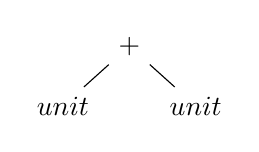
\begin{tikzpicture}[scale=1.2]
    \node {$+$} [grow=down, sibling distance=4.0em, level distance=1.8em]
      child { node {$\text{unit}$} }
      child { node {$\text{unit}$} } ;
  \end{tikzpicture}
  \end{center}

\end{frame}


\begin{frame}{With Sums and Unit We Can Simulate Weekdays}

  \begin{itemize}
    \item We write: $\text{unit} + \text{unit} + \text{unit} + \text{unit} + \text{unit} + \text{unit} + \text{unit}$
    \item We mean: ``A value of this type is either \emph{left}, or
    \emph{right;left}, or \ldots, or \emph{right;right;right;right;right;right}.''
  \end{itemize}

  \begin{center}
  \begin{tikzpicture}[scale=1.0]
    \node {$+$} [grow=down, sibling distance=4.0em, level distance=1.8em]
      child { node {$\text{unit}$} }
      child { node {$+$}
        child { node {$\text{unit}$} }
        child { node {$+$}
          child { node {$\text{unit}$} }
          child { node {$+$}
            child { node {$\text{unit}$} }
            child { node {$+$}
              child { node {$\text{unit}$} }
              child { node {$+$}
                child { node {$\text{unit}$} }
                child { node {$\text{unit}$} }
              }
            }
          }
        }
      }
    ;
  \end{tikzpicture}
  \end{center}

\end{frame}


\begin{frame}{What About Natural Numbers?}

  \begin{itemize}
    \item We would like to have: \\
          ``A value of this type is either \emph{left} or
          \emph{right;left} or \emph{right;right;left} or \ldots''
    \item We would need to write: $\text{unit} + \text{unit} + \text{unit} + \ldots$
  \end{itemize}

  \begin{center}
  \begin{tikzpicture}[scale=1.2
    , and so on/.style={thick, dotted}
    ]
    \node {$+$} [grow=down, sibling distance=4.0em, level distance=1.8em]
      child { node {$\text{unit}$} }
      child { node {$+$}
        child { node {$\text{unit}$} }
        child { node {$+$}
          child { node {$\text{unit}$} }
          child[and so on] { node {} }
        }
      }
    ;
  \end{tikzpicture}
  \end{center}

\end{frame}


\subsection{Inductive Types}

\begin{frame}{Recursive Types to the Rescue!}

  \begin{itemize}
    \item We write: $\mu a . \text{unit} + a$
    \item We mean: ``The least fixed point which satisfies the equation $a = \text{unit} + a$ ''
  \end{itemize}

  \begin{center}
  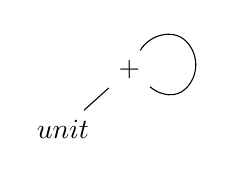
\begin{tikzpicture}[scale=1.2]
    \node (root) {$+$} [grow=down, sibling distance=4.0em, level distance=1.8em]
      child { node {$\text{unit}$} }
      child[missing] {}
    ;
    \draw (root)
     to[out=320, in=225] ($(root) + (0.6, -0.2)$)
     to[out=45, in=315] ($(root) + (0.6, 0.3)$)
     to[out=135, in=60] (root);
  \end{tikzpicture}
  \end{center}

\end{frame}


\begin{frame}{Things We Would Like to Know}

  \begin{itemize}
    \item What is a solution of the equation $a = \text{unit} + a$ ?
    \item Is it a fixed point?
    \item Is it the least fixed point?
    \item Is this still, somehow, the natural numbers?
    \item Can we define an information ordering on this set?
    \item Is this ordering a domain?
  \end{itemize}

\end{frame}


\begin{frame}{How to Answer These Questions?}

  \begin{itemize}
    \item
      What is a solution of the equation $a = \text{unit} + a$ ?
      \begin{itemize}
        \item
          Claim: The set of all finite paths which start at the root and end in
          a leaf
      \end{itemize}
    \item
      How to prove that it is a fixed point?
      \begin{itemize}
        \item
          We need to prove: there are functions
          $\Phi : \llbracket \mu a . \text{unit} + a \rrbracket \arr \llbracket \text{unit} + (\mu a . \text{unit} + a) \rrbracket$
          and
          $\Psi : \llbracket \text{unit} + (\mu a . \text{unit} + a) \rrbracket \arr \llbracket \mu a . \text{unit} + a \rrbracket$
          such that: \\
          $\Phi \circ \Psi = \text{id}$ and $\Psi \circ \Phi = \text{id}$
      \end{itemize}
  \end{itemize}

  \begin{columns}[totalwidth=.7\textwidth]

  \begin{column}{.5\textwidth}
  \begin{center}
    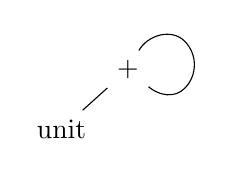
\begin{tikzpicture}[scale=1.2]
      \node (root) {$+$} [grow=down, sibling distance=4.0em, level distance=1.8em]
        child { node {unit} }
        child[missing] {}
      ;
      \draw (root)
       to[out=320, in=225] ($(root) + (0.6, -0.2)$)
       to[out=45, in=315] ($(root) + (0.6, 0.3)$)
       to[out=135, in=60] (root);
    \end{tikzpicture}
  \end{center}
  \end{column}

  \begin{column}{.5\textwidth}
  \begin{center}
    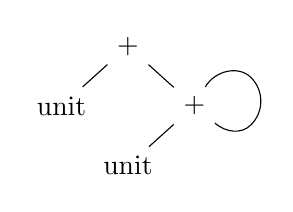
\begin{tikzpicture}[scale=1.2]
     \node (root) {$+$} [grow=down, sibling distance=4.0em, level distance=1.8em]
        child { node {unit} }
        child { node (plus) {$+$}
          child { node {unit} }
          child[missing] {}
        }
      ;
      \draw (plus)
       to[out=320, in=225] ($(plus) + (0.6, -0.2)$)
       to[out=45, in=315] ($(plus) + (0.6, 0.3)$)
       to[out=135, in=60] (plus);
    \end{tikzpicture}
  \end{center}
  \end{column}

  \end{columns}

\end{frame}


\begin{frame}{Foobar}

 \begin{itemize}
  \item How to prove that we have a least fixed point?
  \item What is an information ordering?
  \item What is a domain?
 \end{itemize}

\end{frame}


\subsection{Coinductive Types}

\begin{frame}{Fixpoint Enlargement Right Now}

  \begin{itemize}
    \item Claim: $\nu a . \text{unit} + a$, that is: The set of all paths that start
          at the root and either end at an arbitrary node or are infinite, is
          the \emph{largest} fixed point of $a = \text{unit} + a$.
    \item Is it a fixed point?
    \item Is it the largest fixed point?
    \item How does it relate to the natural numbers?
    \item Can we define an information ordering on this set?
    \item Is this ordering a domain?
  \end{itemize}

\end{frame}


\section{The Plan}

\subsection{The Coinductive Natural Numbers With Computation Steps}

\begin{frame}{The Coinductive Natural Numbers With Computation Steps}

  \begin{itemize}
    \item
      Let's consider $\nu a . \text{unit} + a + a$
    \item
      Three constructors $0 : a$, $S : a \arr a$, $\_ : a \arr a$
    \item
      Values are
      \begin{itemize}
        \item infinite sequences of $S$ and $\_$
        \item finite sequences of $S$ and $\_$, terminated by $0$
      \end{itemize}
  \end{itemize}

  \begin{center}
  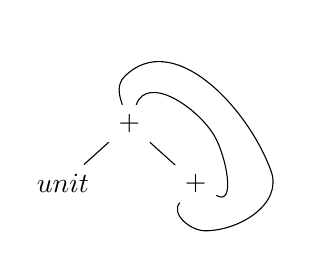
\begin{tikzpicture}[scale=1.2]
    \node (root) {$+$} [grow=down, sibling distance=4.0em, level distance=1.8em]
      child { node {$\text{unit}$} }
      child { node (plus) {$+$} };
    \draw (plus) to [out=330, in=300] ($(plus) + (0.2, 0.5)$)
                 to [out=120, in=70] (root);
    \draw (plus) to [out=230, in=180] ($(plus) + (0.1, -0.5)$)
                 to [out=0, in=290] ($(root) + (1.5, -0.5)$)
                 to [out=110, in=45] ($(root) + (-0.05, 0.5)$)
                 to [out=225, in=110] (root)
    ;
  \end{tikzpicture}
  \end{center}

\end{frame}


\section*{Summary}

\begin{frame}{Summary}

  \begin{itemize}
  \item
    Recursive datatypes are type expressions of the form $a = t(a)$
  \item
    $\mu a . t$ and $\nu a . t$ denote the least and largest fixed points of such equations
  \item
    My plan is to answer some questions regarding $\nu a . \text{unit} + a + a$
  \end{itemize}

\end{frame}


\end{document}


